\section{Periodic Motion}

\makelabheader %(Space for student name, etc., defined in master.tex or labmanual_formatting_commands.tex)

{\bf Objectives }

\begin{itemize}
\item To learn directly about some of the characteristics of periodic motion, namely period, frequency, and amplitude. 
\item To investigate the relationships between position, velocity, acceleration, and force in simple harmonic motion. 
\item To investigate energy in simple harmonic motion.
\end{itemize}
\textbf{Introduction }

Periodic motion is motion that repeats itself. You can see the repetition in
the position-, velocity-, or acceleration-time graphs. The length of time to
go through one cycle and begin to repeat the motion is called the period. The
number of cycles in each second is called the frequency. The unit of frequency,
cycles per second, is given a special name --- Hertz.

\textbf{Motion of a Mass Hanging from a Spring} 

In this unit you will investigate the motion of a mass hanging from a spring.

\textbf{Apparatus} 

\begin{itemize}
\item Support with cross bar
\item Force probe
\item Large spring
\item Motion detector 
\item Variety of masses 
\item Pasco 550 Interface
\item \textit{Capstone} software (\filename{P\_V\_Graphs.cap} and \filename{SHM.cap} experiment files)
\end{itemize}
\textbf{Activity 1: Periodic Motion of a Mass-Spring System} 

(a) Open the file \filename{P\_V\_Graphs.cap} in the \filename{\coursefolder} folder. Hang the large spring from the force probe hook with the large diameter coils down and hang a 200-g mass from the spring. (Remember to calibrate the force probe) Place the motion detector facing up directly below the spring. Pull the mass straight downward about 10 cm, and let go. 
Adjust the height of the support so that the mass comes no closer than 15 cm 
to the detector. Record data for a few seconds to display position-time and 
velocity-time graphs of the motion. Sketch the graphs on the following axes.

\vspace{0.3cm}
{\par\centering 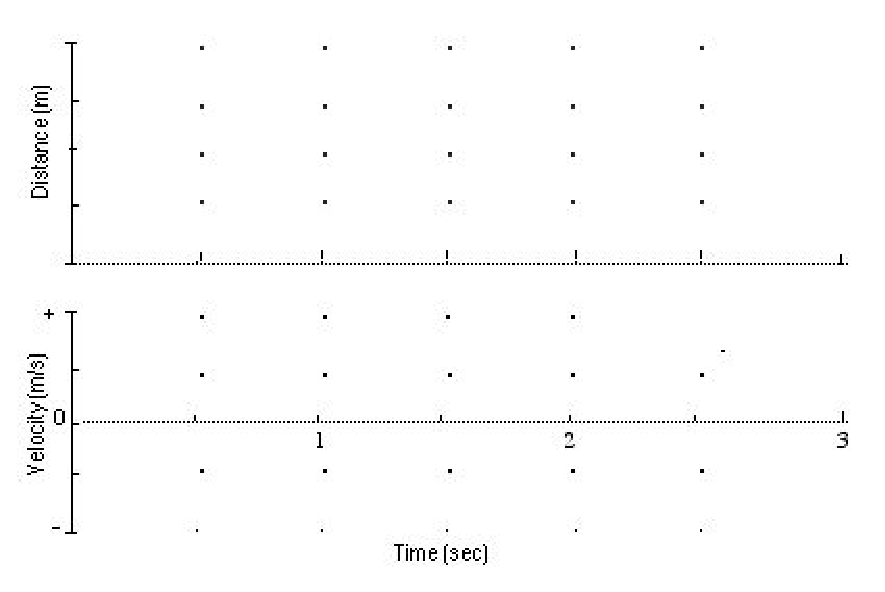
\includegraphics{periodic_motion/periodic_motion_fig1.eps} \par}
\vspace{0.3cm}

\textbf{Comment}: Note that when an object returns to the same position, it 
does not necessarily mean that a cycle is ending. It must return to the same 
position, and the velocity and acceleration must also return to the same 
values in both magnitude and direction for this to be the start of a new cycle. 

%(b) Label the graphs above with: ``B'' at the Beginning of a
%cycle and ``E'' at the End of the same complete cycle. ``A''
%on each spot where the mass is moving Away from the detector fastest. ``T''
%on each spot where the mass is moving Toward the detector fastest. ``S''
%on each spot where the mass is standing Still. ``F'' where the
%mass is Farthest from the motion detector. ``C'' where the mass
%is Closest to the motion detector.

(b) Do the position and velocity graphs appear to have the same period? Do their
peaks occur at the same times? If not, how are the peaks related in time, i.e. 
what fraction of a period is their phase difference?
\vspace{20mm}

(c) Use the \textbf{Delta Tool} to measure the period of the motion. (For
better accuracy, measure the total time over as many cycles as possible and
divide by the number of cycles.)
\vspace{20mm}

(d) Using the \textbf{Statistics} function, determine and record the maximum and minimum 
displacement.  Determine the amplitude of the motion from $A = (x_{\rm max} - x_{\rm min})/2$.
\vspace{30mm}

(e) Save the graph. You will be using it again in Activity 7.

\newpage

\textbf{Simple Harmonic Motion }

The motion of a mass hanging from a spring that you looked at in Activity 1
is a close approximation to a kind of periodic motion called simple harmonic
motion (sometimes abbreviated SHM).

\textbf{Activity 2: Predictions:  What Factors Determine the Period of the Mass-Spring System? }

What can you do to change the period of the SHM of the mass-spring system? What
will happen to the period if you increase the amplitude? Increase the mass?
Increase the spring constant (use a stiffer spring)?
\vspace{30mm}

\textbf{Activity 3: The Period of SHM and the Amplitude} 

(a) Repeat the procedure of Activity 1, but with a different starting position
(other than 15 cm). (Warning: Do not make the amplitude so large that the mass
comes closer than 0.15 m from the motion detector.) When you have good graphs,
find and record the period and the amplitude using the methods described in
Activity 1. 
\vspace{20mm}

%(b) Take ratios of the period and the amplitude of Activity 1 to those 
%determined here.
%\vspace{20mm}

(b) Is there evidence that the period depends on amplitude? (Did the change
in amplitude result in a comparable change in period?) How does this
compare with your prediction?
\vspace{30mm}

\textbf{Activity 4: The Dependence of the Period of a SHM on the Mass} 

(a) Carefully measure the period for four other masses. Record the masses and
the measured periods in a table in the space below along with the mass and 
period from Activity 1. \textbf{Note:} Add half the mass of the spring to each
mass value. This accounts for the fact that the theory of SHM neglects the mass 
of the spring.
\vspace{35mm}

(b) Does the period depend on the mass? Does it increase or decrease as mass
is increased?
\vspace{15mm}

(c) Determine the mathematical relationship between the period $T$ and the mass
$m$ by finding a function that fits the data. Do this by using \textit{Excel} to plot 
a graph of $T$ vs $m$ (use the TOTAL mass including half the mass of the 
spring) and fitting the data with a POWER function. Write the equation that 
provides the best fit to the data in the space below. What is the power of 
$m$ for your best fit? Print the graph and include with this unit.
\answerspace{20mm}

\textbf{Comment:} You should have found that $T$ is independent of amplitude 
and proportional to \( \sqrt{m} \). The actual expression for the period is
\[T=2\pi \sqrt{\frac{m}{k}.}\]


\textbf{Velocity, Acceleration, Force and Energy }

In this investigation you will look more carefully at the distance, velocity
and acceleration graphs for simple harmonic motion. You will also look at the
force graph, and will examine the energy associated with simple harmonic motion.

\textbf{Activity 5: Determination of the Spring Constant }

Measure the distance the spring stretches for four different masses and use
these data to determine the spring constant, $k$, as you did in either the Work and Kinetic Energy experiment or the Hooke's Law experiment. Record your data and the result for $k$ in the space below.
\answerspace{40mm}

\textbf{Activity 6: Velocity, Acceleration, and Force for SHM} 

(a) Consider the motion you looked at in Activity 1 when the mass was 200 g
and the initial position was 15 cm. Sketch the position and velocity graphs
that you observed on the axes below using dashed lines.

\vspace{0.3cm}
{\par\centering 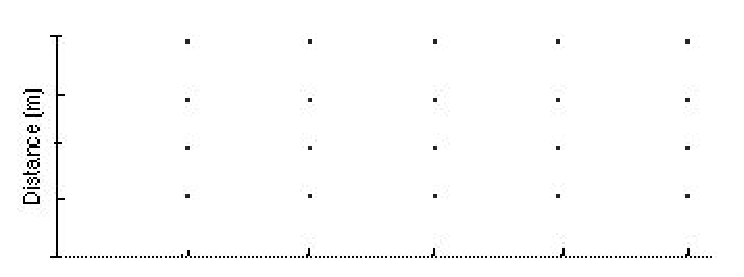
\includegraphics{periodic_motion/periodic_motion_fig2.eps} \par}
\vspace{0.3cm}

\vspace{0.3cm}
{\par\centering 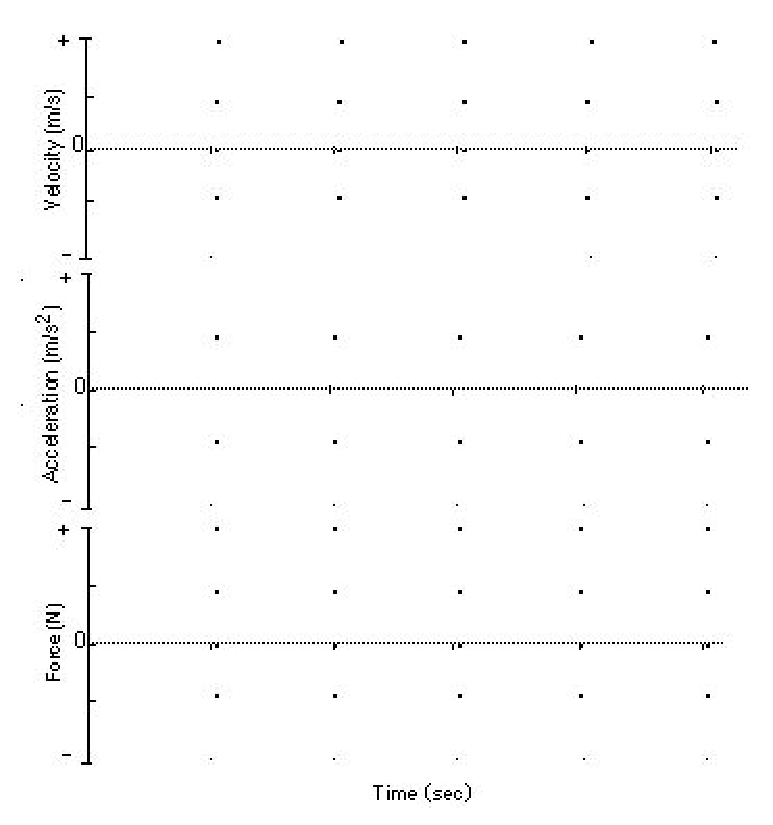
\includegraphics{periodic_motion/periodic_motion_fig3.eps} \par}
%\vspace{0.3cm}

(b) Based on what you know about the relationships between velocity, 
acceleration, and force, use dashed lines to sketch your predictions for the 
acceleration and force graphs.

(c) Suspend the 200-g mass from the spring and open the file \filename{SHM.cap} in the \filename{\coursefolder} folder. Calibrate the force probe (see Appendix~\ref{capstone}).
Start the mass oscillating with an amplitude of 15~cm and record data for a few seconds.
When you have obtained good graphs, sketch the results on the above axes using
solid lines. Print your graph and attach to this unit.

(d) When the mass is at its maximum distance from the detector, is the absolute
 value of the velocity
maximum, minimum or some other value according to your graphs? Does this agree
with your predictions? Does this agree with your observations of the oscillating
mass? Explain.
\answerspace{15mm}

(e) When the mass has its maximum positive velocity, is its distance from the
detector maximum, minimum, the equilibrium value or some other value according
to your graphs? What about when it reaches maximum negative velocity? Does this
agree with your predictions? Does this agree with your observations of the 
oscillating mass? Explain. 
\answerspace{10mm}

\pagebreak[2]
(f) According to your graphs, for what distances from the detector is the 
acceleration maximum? For what distances is the acceleration zero? What is the 
velocity in each of these cases?
\answerspace{20mm}

(g) Compare the force and acceleration-time graphs. Describe any similarities.
Does the force graph agree with your prediction?
\answerspace{20mm}

(h) From your graphs, what would you say is the relationship between force and
acceleration? 
\answerspace{20mm}

(i) Compare the force and distance(position)-time graphs. What would you say
is the relationship between force and position? 
\answerspace{20mm}

\textbf{Activity 7: Energy of a Mass Undergoing SHM }

Now use the graphs from Activity 1 to examine the energy relationships
in simple harmonic motion. To do this you will need to print the graphs and draw a horizontal line through the equilibrium position on the position vs time graph.  $x$ values must be determined relative to this equilibrium position (which represents a displacement of zero).

(a) At what points is the kinetic energy of the mass zero? Label these points
on your distance and velocity graphs above with a K.

(b) Calculate the elastic potential energy due to the spring at one of these
points. Label the point you use on your velocity and distance graphs with a
1. Use $U = \frac{1}{2}kx^{2}$, where  $x$ is the distance from the equilibrium 
position and $k$ is the force constant of the spring, which you have already 
measured. Use the \textbf{Delta Tool} to measure position, then subtract the 
equilibrium position to determine $x$. Show your data and calculations 
in the space below. 
\answerspace{20mm}

(c) At what points is the potential energy zero? Label these points with a P
on your distance and velocity graphs.

(d) If you measured the kinetic energy at one of these points, what would you
expect its value to be? Explain.
\answerspace{15mm}

\pagebreak[2]
(e) Check your prediction. Calculate the kinetic energy at one of these points.
Label the point you use on your velocity graph with a 2. Use 
$K = \frac{1}{2} mv^{2}$, where $m$ is the total mass including half the mass of 
the spring. Use the \textbf{Delta Tool} to determine $v$. Show your data and 
calculations in the space below.
\vspace{20mm}

(f) Did your calculated kinetic energy agree with your prediction?
\vspace{15mm}

(g) If you calculated the potential and kinetic energies at a point where 
neither of these was zero, what would you expect the total energy to be? 
Explain.
\vspace{20mm}

(h) Check your prediction. Make a table below with headings for $v$~(m/s), 
position ($m$), $x$~(m) where $x$ is the difference between the position
of the mass and the equilibrium position, $K$, $U$, and the total energy.
Pick 5 or 6 points where the mass has both kinetic and
potential energy, calculate them both ($K$ and $U$), and then calculate the 
total energy for each point ($K+U$). Label these points on your distance
and velocity graphs with numbers. 
Make a histogram of your results for the total energy and calculate the 
average and standard deviation.
For information on making histograms, see \textbf{Appendix \ref{excel}}. For information 
on calculating the average and standard deviation, see \textbf{Appendix \ref{treatment}}. 
Record the average and standard deviation here.
Attach the histogram to this unit.
\vspace{60mm}

(i) What does the histogram of the total energy tell you? Be quantitative in 
your answer.
\vspace{20mm}

(j) Is the total energy conserved?  Be quantitative in your answer.

